% Chapter 3

\chapter{System Overview} % Main chapter title

\label{systemoverview} % For referencing the chapter elsewhere, use \ref{Chapter1} 

\lhead{Chapter 3. \emph{System Overview}} % This is for the header on each page - perhaps a shortened title

%----------------------------------------------------------------------------------------

\section{Introduction}

The Context-Aware Guide (subsequently called "CA Guide" or simply "Guide") needs to be defined to fit indoor, outdoor and mixed sites, like classical museums, parks and gardens. 
The basic functionality must be accessible even by persons not familiar with mobile technology. The context awareness techniques can help avoiding big parts of explicit user input, allowing the visitor to focus completely on it's environment without reading and typing numbers.

This thesis, however, focuses on the technical foundation of the whole system, and thus on the system architecture on several levels of abstraction. 

The following figure shows a high level view of the complete system, consisting of the visitor guide front-end running on a mobile device, a back-end for the modelling the guide and performing analytic functions. The database server is accessed by both system parts and represents the communication basis - there is no direct communication between font and back end. All data is exchanged over the database, enabling asynchronous communication.

As database server Couchbase was chosen due to it's automatic synchronization capabilities, it's mobile version and it's ability to scale out without completely redesigning the way the database is accessed by the application.\footnote{After actually having reached the limits of scalabity of a single classical relational database server of a commercial project and painfully distributing the database on several servers of the productive system, the idea of an easy scale out using a NoSql database and map-reduce queries seemed even more ingenious to me.} 

\begin{figure}[H]
\centering
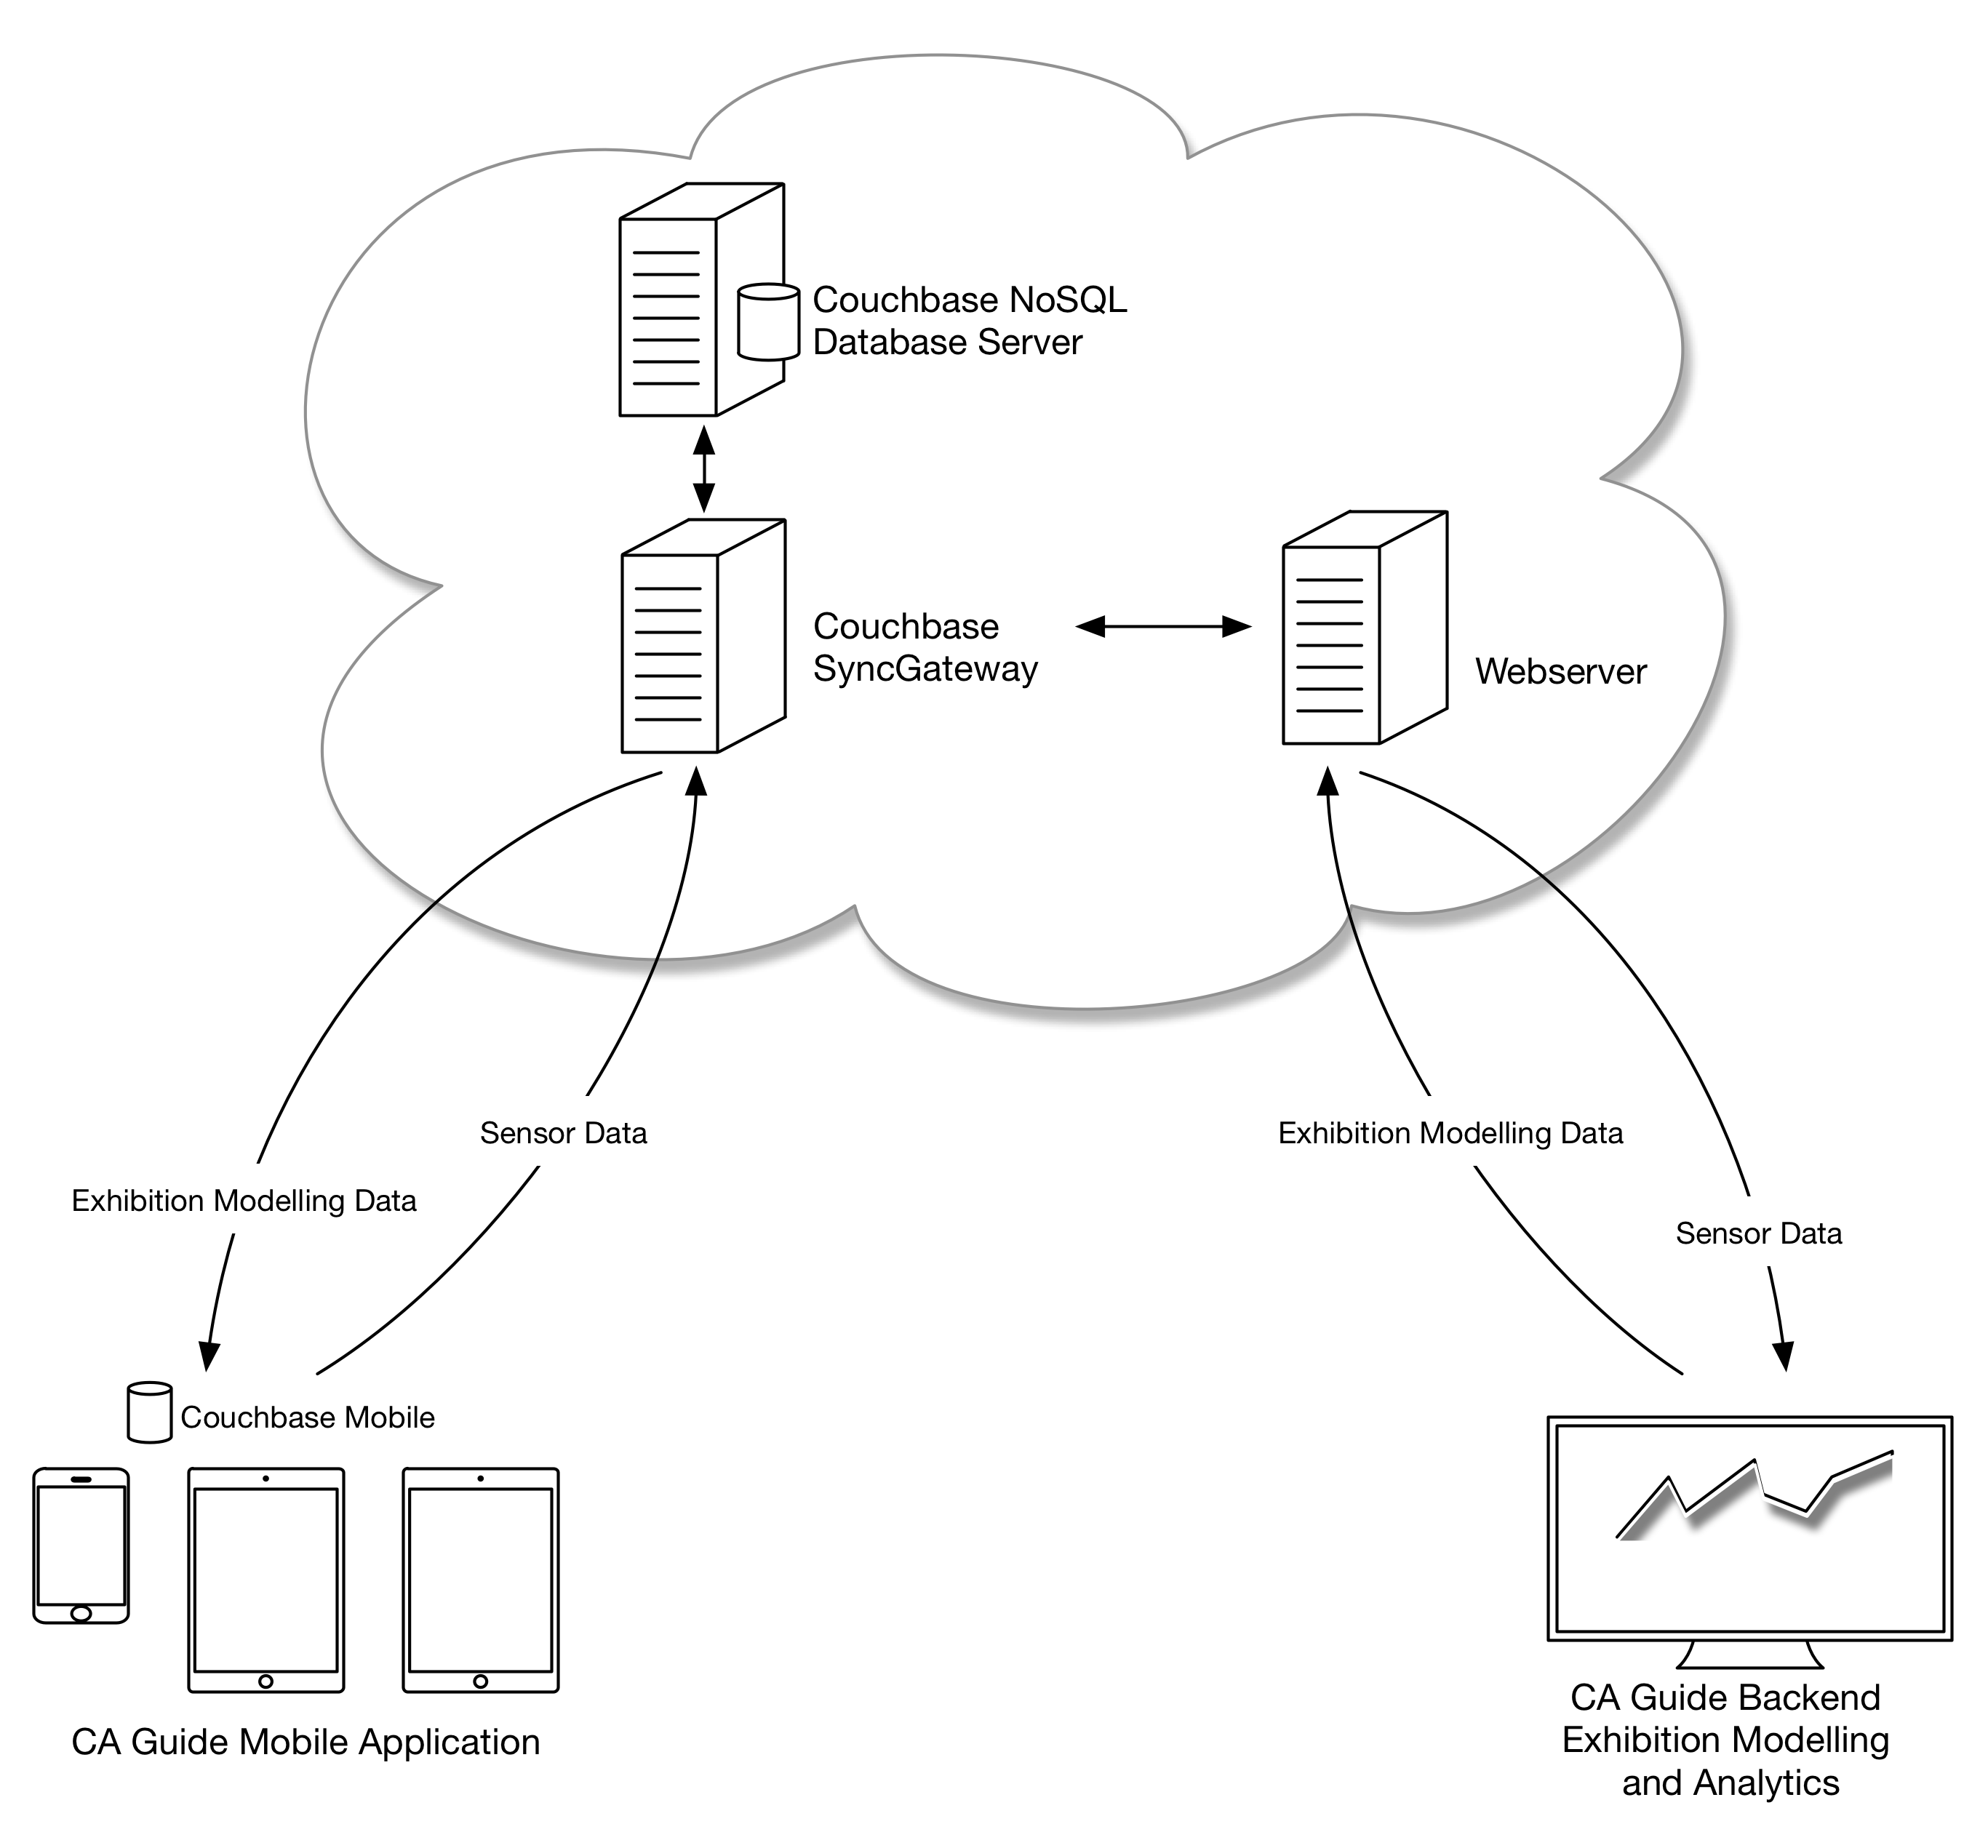
\includegraphics[height=0.8\textwidth]{system-overview}
\caption{CA Guite Architecture Overview}
\end{figure}

%Image Mockup CA Guide 
%Image A Backend Screen Mockup

The two system parts share a unique data structure for the site model containing all data needed for the mobile guide and the sensor traces, containing recorded raw or computed measurements at different time intervals. Thus, before starting with the front or back-end, it is important to reason about the common data model.

\section{Data Model}

\subsection{Site Modelling}

A single park or museum is modeled using the JSON data format. Compared to XML, JSON is more readable, easier to produce without dedicated tools in a simple text editor and more compact, mainly on account of the elimination of duplicated entity names in closing tags.

The main entities used for modeling a site are shown on the following picture.

\begin{figure}[H]
\centering
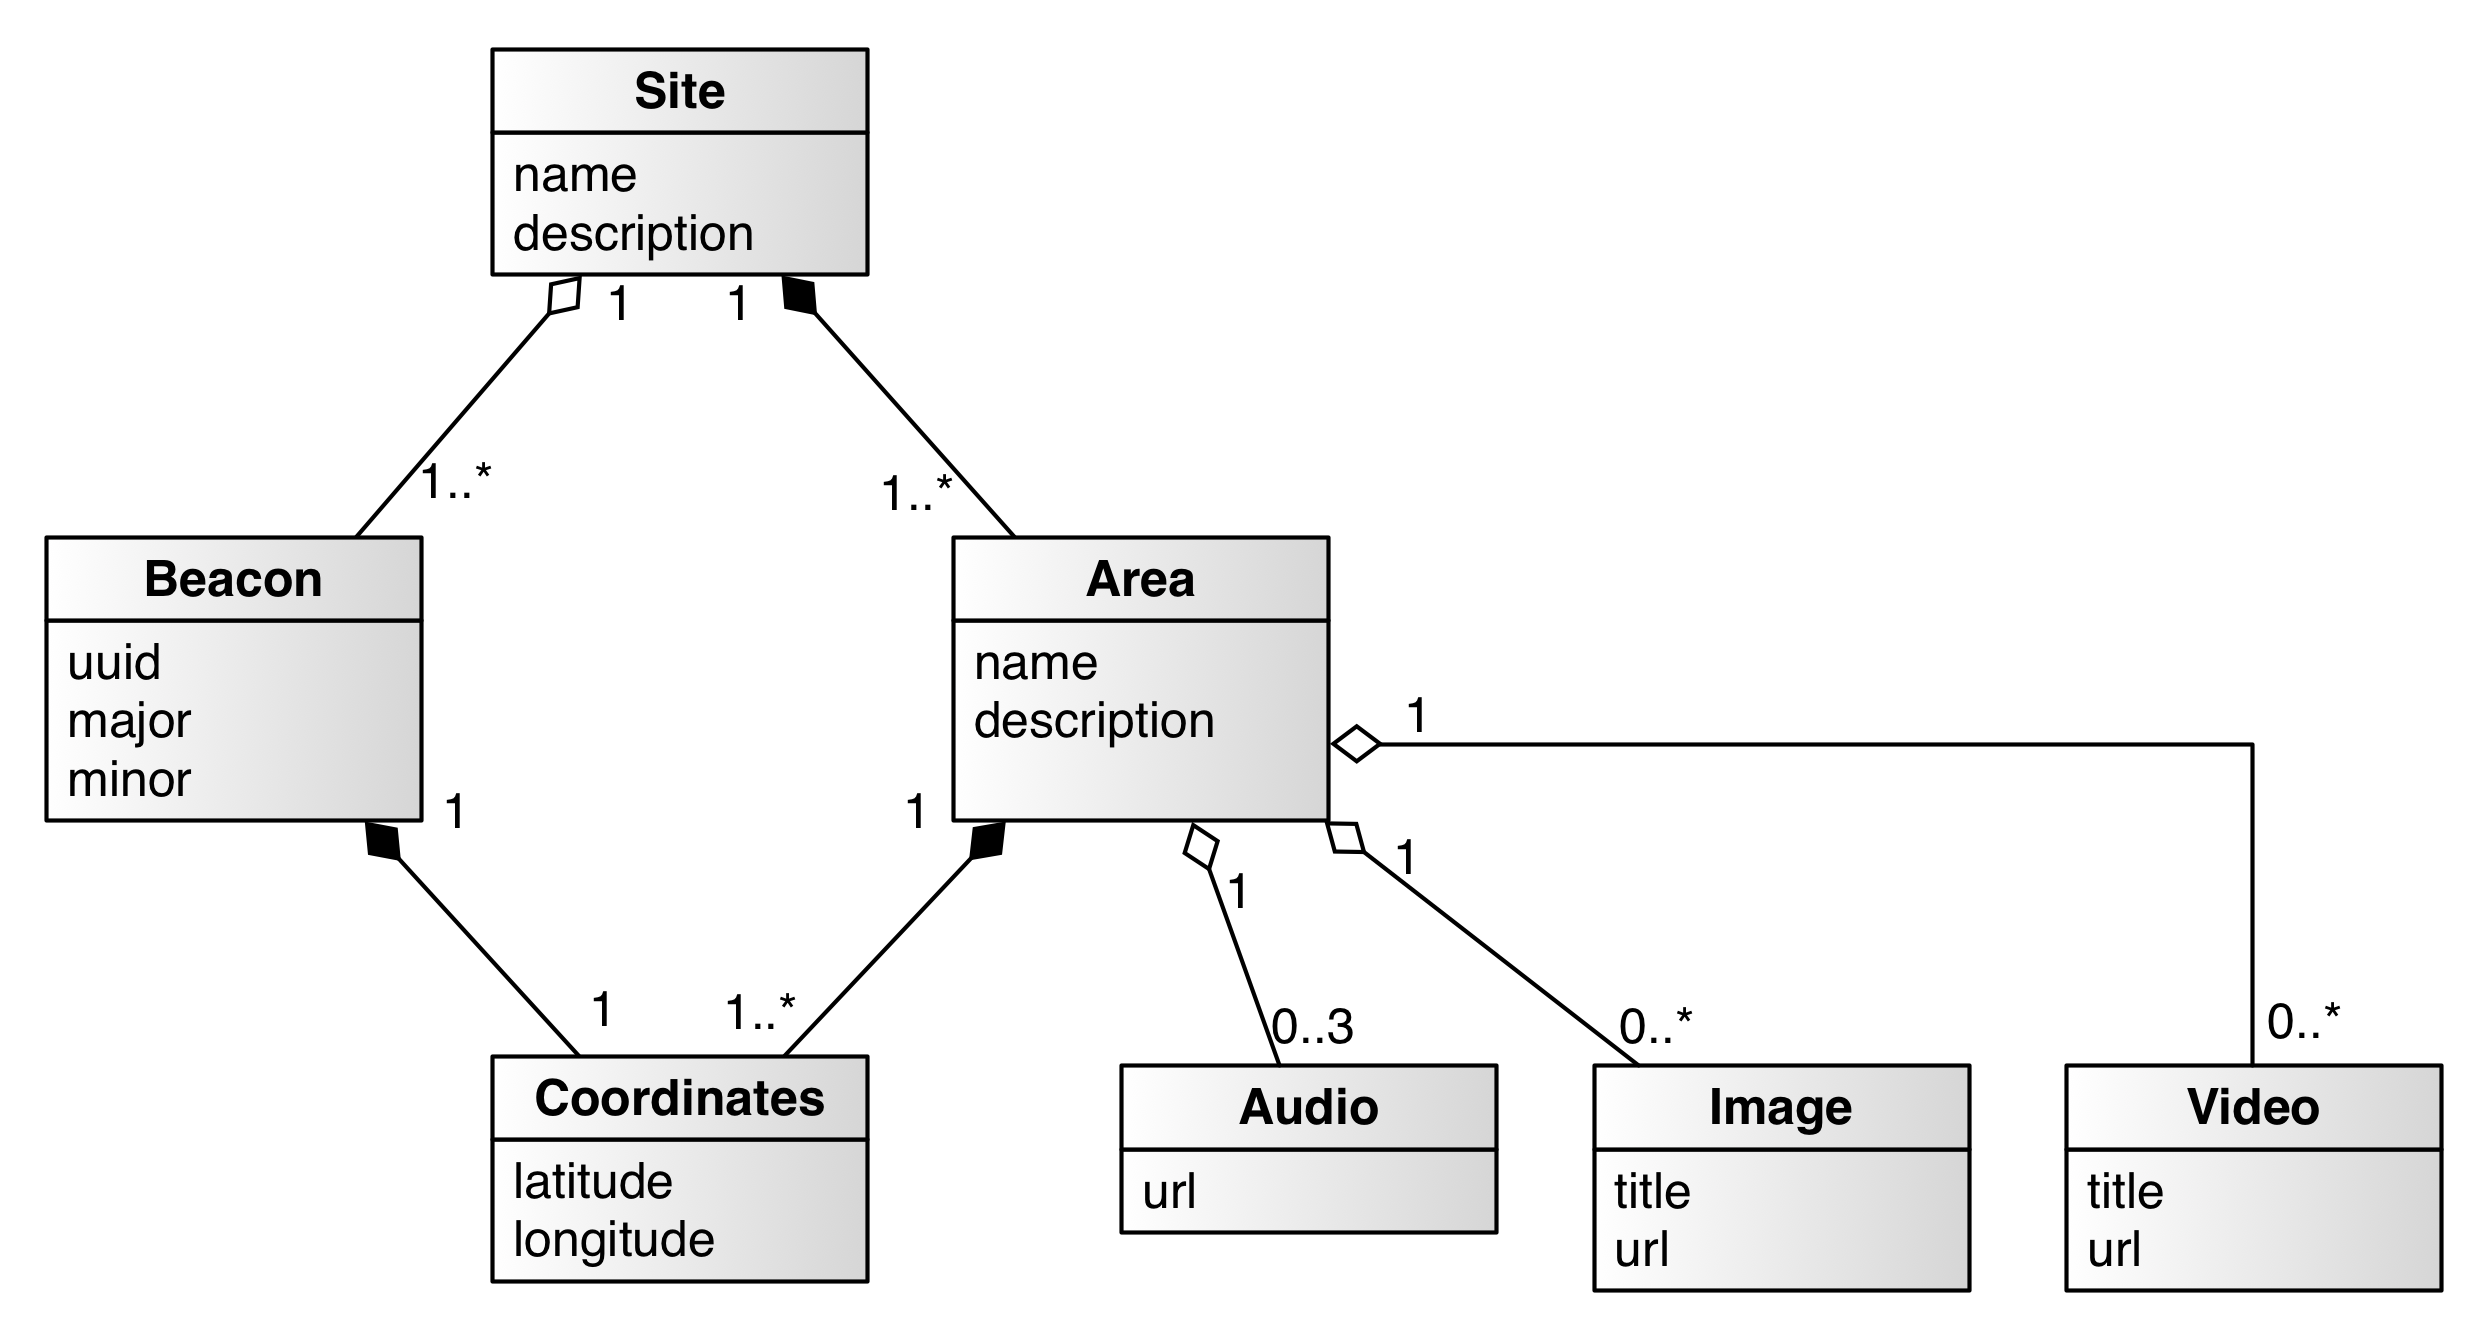
\includegraphics[height=0.5\textwidth]{data-model-site}
\caption{Data model of a site (using UML notation)}
\end{figure}

A site is composed of several areas, geographically delimited by a list of coordinates. For indoor sites, several beacons can be added with their identifying properties and the defined position. Beacons are decoupled from areas in the data model. They are a positioning help\footnote{After the mobile front-end determined it's (indoor) position based on the beacon's data, it identifies the area it is situated using geometrical computations} that could be replaced in the future.
An area has a textual description and optionally (even though in productive systems very likely) up to three audio files containing explanations as voice recordings and other fitting audio material. These three files reflect a rising level of detail. 
Furthermore, several images and videos can be added to the area.

With a normal relational database, pretty much of the entities would be saved in separate tables in a normalized way using primary and foreign keys to represent the relationships between the tables. In case of the one to many relation between an area and it's images, the usual way is to define a separate table "Image" and to store the image or an url beside the areas id they belong to.

With a document-oriented database, data is commonly stored in a more aggregated way. In contrast to the records of a relational database's, records of document-oriented database have a more complex structure allowing lists and nesting. In \cite{nosqldistilled}, the authors suggest the term "aggregate" for these records. They adopted this term from \cite{domaindriven} "Domain-Driven Design". An aggregate is a set of objects used together. That means they are loaded and saved to the database as a unit and they determine the unit to be locked for the management of consistency.  

As is often the case, there is not only one right solution. The precise level of aggregation depends mainly on how the data will be accessed later. 

From a site modeling point of view at the back-end, single areas and single beacons can be viewed as aggregates, allowing more granular modifications and enabling collaborative editing of a single site.
From a front-end point of view, a whole site definition can be regarded an aggregate. During initialization, the whole site is read with all areas and beacons. This can be done with a single database query. On the mobile device, sites are only read and never modified.
 

The following JSON-document shows a simplified site aggregate containing one area and one beacon.

\begin{lstlisting}
key: "site-CXN01"
value: {
 "type":"city",
 "name":"Konstanz",
 "description":"",
 "areas": [{
     "id":"area-51",
     "type":"area",
	 "name":"Konstanz Cathedral", 
	 "description":"A historical building in Konstanz, ...",
	 "locationDefinition": {
	 	"type": "polygon",
	 	"coordinates": [{"lat":47.663093, "lon":9.176371},{"lat":47.663336, "lon":9.175215},{"lat":47.663673, "lon":9.176075}],
	 	"floor": 1
	 }, 
	 "images":["cathedral-panorama.png","cathedral-north-west.png"], 
	 "audio":{
	 	"level1": "cathedral-1.mp3",
	 	"level2": "cathedral-2.mp3",
	 	"level3": "cathedral-3.mp3"
	 }, 
	 "videos":[]}],
  "beacons":  [{
  	"id":"beacon-42",
  	"uuid":"F7826DA6-4FA2-4E98-8024-BC5B71E0893E",
  	"major":"40231",
  	"minor":"203",
  	"coordinates": {"lat":47.663278, "lon":9.176214}
  }]
}
\end{lstlisting}

Although NoSQL databases are schema-less, it's important to keep in mind that there still is an implicit data structure the application relies on. The risk of malformed data ca be handled with automated tests. In case of manually produced JSON documents, a JSON Schema can be used for asserting a valid structure of a JSON file, similar to a DTD (Data Type Definition) in XML (http://json-schema.org).

\subsection{Sensor Data}

Sensor data is saved to the Couchbase database to allow replaying it for development, testing, presentations and for analytics presented in the system's web backend. 

The single measurements can be very high frequent, for example in case of accelerometer data, that is updated every 10 millisecons. New beacon measurements are available every second. Events on a higher logical level, like "entering region a", will occur less frequently.

\begin{lstlisting}[basicstyle=\footnotesize]
key: SENSORTRACE-CXN01
value: {
  "date": "2015-02-12",
  "time": "20:15",
  "accelerometer": [
    {"timestamp": 12345678.35, "data": [1.235, 0.364, 0.021]},
    {"timestamp": 12345678.40, "data": [1.217, 0.378, 0.009]},
    ...
  ],
  "gyroscope": [
    {"timestamp": 12345678.35, "data": [1.235, 0.364, 0.021]},
    {"timestamp": 12345678.40, "data": [1.217, 0.378, 0.009]},
    ...
  ],
  "magnetometer": [
    {"timestamp": 12345678.35, "data": [1.235, 0.364, 0.021]},
    {"timestamp": 12345678.40, "data": [1.217, 0.378, 0.009]},
    ...
  ],
  "beacons": [
    {"timestamp": 12345679.05, "data": [["A3F3", -51],["85B7", -68]]},
    {"timestamp": 12345680.05, "data": [["A3F3", -51],["85B7", -68]]},
    ...
  ],
  "gps": [
    {"timestamp": 12345679.35, "data": [1.44, 10.021]},
    {"timestamp": 12345680.36, "data": [1.44, 10.009]},
    ...
  ],
}
\end{lstlisting}


\section{Setting up the Couchbase Server Infrastructure}

Couchbase Server
Admin Port

Couchbase Sync Gateway
config.json

%Backend has two databases, work in progress in couchbase NoSQL, aggregates site area beacon, site aggregate published over sync-gateway